\begin{figure*}[!ht]
    \centering
    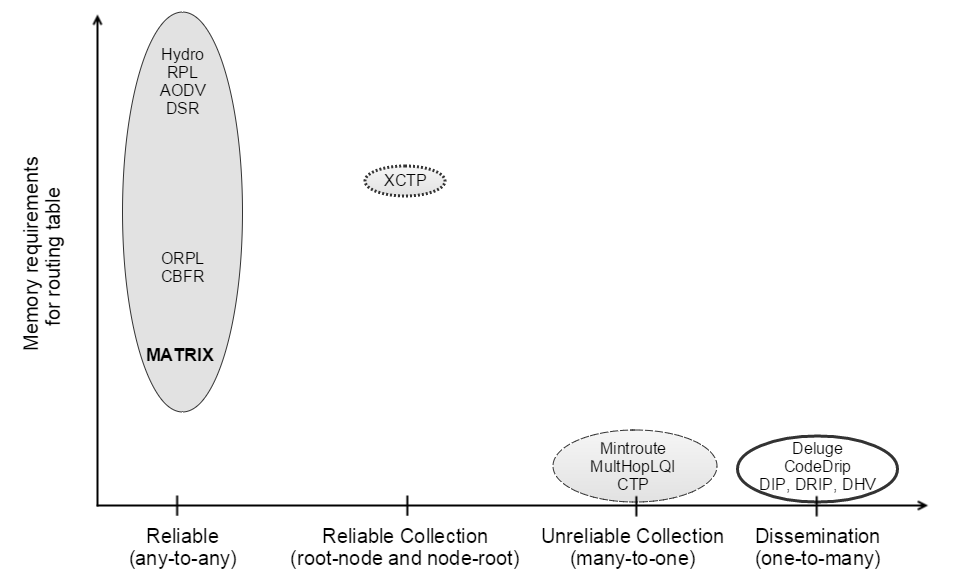
\includegraphics[width=0.75\linewidth]{Images/overview.png}
    \caption{Overview of related works}
    \label{fig:overview-rel}
\end{figure*}

\section{Related Work}
\label{sec:related}

%\begin{table*}[ht]
\centering
\caption{Protocols comparison}
\label{tab:comparative}
\resizebox{\textwidth}{!}{%
\begin{tabular}{@{}lccccc@{}}
\toprule
\multicolumn{1}{c}{{\bf Protocols}} & {\bf \begin{tabular}[c]{@{}c@{}}Ipv6\\ compatible\end{tabular}} & {\bf \begin{tabular}[c]{@{}c@{}}Routing table\\ memory size\end{tabular}}                                                 & {\bf \begin{tabular}[c]{@{}c@{}}Communication\\ Paradigm\end{tabular}}                           & {\bf \begin{tabular}[c]{@{}c@{}}Adaptative \\ beacon\end{tabular}} & {\bf \begin{tabular}[c]{@{}c@{}}Latency\\ (worst case for anycast)\end{tabular}}                           \\ \midrule
AODV, DYMO                          & \ding{53}                                                     & High                                                                                                                      & Any-to-any                                                                                       & \ding{53}                                                        & \begin{tabular}[c]{@{}c@{}}High\\ (Finding route)\end{tabular}                                             \\
DSR                                 & \ding{53}                                                     & High                                                                                                                      & Any-to-any                                                                                       & \ding{53}                                                        & \begin{tabular}[c]{@{}c@{}}High\\ (Finding route)\end{tabular}                                             \\
Hydro                               & \ding{53}                                                     & \begin{tabular}[c]{@{}c@{}}High\\ (table for routes and flows)\end{tabular}                                                & Any-to-any                                                                                       & \ding{53}                                                        & \begin{tabular}[c]{@{}c@{}}Middle\\ (Need request to\\ border node)\end{tabular}                           \\
RPL                                 & \ding{52}*                                                     & \begin{tabular}[c]{@{}c@{}}High\\ (table entry for each \\ descendant node)\end{tabular}                                  & Any-to-any                                                                                       & \ding{52}                                                        & \begin{tabular}[c]{@{}c@{}}Middle\\ (Need request to \\ sink)\end{tabular}                                 \\
ORPL                                & \ding{52}*                                                     & Middle                                                                                                                    & Any-to-any                                                                                       & \ding{52}                                                        & \begin{tabular}[c]{@{}c@{}}Middle\\ (Need request to\\ sink)\end{tabular}                                  \\
CBFR                                & \ding{53}                                                     & Middle                                                                                                                    & Any-to-any                                                                                       & \ding{53}                                                        & --                                                                                                         \\
{\bf MATRIX}                        & Full Ipv6 \ding{52}**                                                          & \begin{tabular}[c]{@{}c@{}}Low\\ (limited by neighborhood)\end{tabular}                                                   & Any-to-any                                                                                       & \ding{52}                                                        & \begin{tabular}[c]{@{}c@{}}Low\\ (Need find mutual\\ parent)\end{tabular}                                  \\
XCTP                                & \ding{53}                                                     & \begin{tabular}[c]{@{}c@{}}Middle\\ (only install routes for active flows and \\remove underutilized entries)\end{tabular} & \begin{tabular}[c]{@{}c@{}}Root-to-nodes\\ and\\ Nodes-to-root\\ (allow any-to-any)\end{tabular} & \ding{52}                                                        & \begin{tabular}[c]{@{}c@{}}Low\\ (Need find mutual\\ parent)\end{tabular}                                  \\
CTP                                 & \ding{53}                                                     & \begin{tabular}[c]{@{}c@{}}Very Low\\ (only parent node)\end{tabular}                                                     & Many-to-one                                                                                      & \ding{52}                                                        & \ding{53}                                                                                                \\
MultiHopLQI                         & \ding{53}                                                     & \begin{tabular}[c]{@{}c@{}}Very Low\\ (only parent node)\end{tabular}                                                     & Many-to-one                                                                                      & \ding{53}                                                        & \ding{53}                                                                                                \\
Minroute                            & \ding{53}                                                     & \begin{tabular}[c]{@{}c@{}}Very Low\\ (only parent node)\end{tabular}                                                     & Many-to-one                                                                                      & \ding{53}                                                        & \ding{53}                                                                                                \\ \midrule
                                    & \multicolumn{1}{l}{}                                            & \multicolumn{1}{l}{}                                                                                                      & \multicolumn{1}{l}{}                                                                             & \multicolumn{1}{l}{}                                               & \multicolumn{1}{l}{\begin{tabular}[c]{@{}l@{}}* Ipv6 can be defined, \\ but only fixed away.\end{tabular}} \\
                                    & \multicolumn{1}{l}{}                                            & \multicolumn{1}{l}{}                                                                                                      & \multicolumn{1}{l}{}                                                                             & \multicolumn{1}{l}{}                                               & \multicolumn{1}{l}{** One-hop DHCPv6.}                                                                      
\end{tabular}
}
\end{table*}

Figure~\ref{fig:overview-rel} shows a qualitative overview of the protocols by highlighting memory requirements for routing table (y-axis) and communication paradigms (x-axis). The latter is divided into: (i) \textit{unreliable}, that only provides unidirectional routes, and (2) \textit{reliable}, that provides bidirectional routes between any pair of nodes in the network supporting, for example, development of reliable end-to-end transport protocols for L2Ns \cite{flush, RCRT, STCP, xctp}.

As shown in Figure~\ref{fig:overview-rel}, MATRIX is a reliable any-to-any protocol with a small memory requirement for routing table. Once MATRIX runs on top of a routing protocol, its cost depends on the underlying routing protocol. We use CTP, a collection protocol, as routing protocol in our implementation. Each node running MATRIX protocol is able to perform any-to-any communication. MATRIX does that by storing at the routing tables only the direct children of the node in the acyclic topology. This makes memory requirements small while allowing any-to-any routing as well as others state-of-the-art protocols. Besides, MATRIX enables IPv6 over sensor network unlike most of the mentioned protocols. To do this, MATRIX uses MHCL protocol \cite{mhcl}, described in Section \ref{sec:mhcl}.

CTP and eXtend CTP~\cite{xctp} are related protocols. CTP is an efficient data collection protocol that uses 4-bit \cite{fonseca2007four} metric to estimate the link quality and route cost. Data and control packets are used to obtain the link quality on CTP. MultiHopLQI~\cite{MultiHopLQI} and MintRoute~\cite{mintroute} have the same propose of CTP, but CTP overcome them as shown in~\cite{Fonseca:2009}. XCTP is an extension of CTP. Besides creating unicast routes to a data collection point, XCTP also creates unicast routes from the root to the sensors. In~\cite{xctp}, the authors argue that XCTP is a reliable collection protocol, in which any-to-any routes are possible and its robustness is maintained when facing topology changes. The authors also show that XCTP requires less memory than other protocols like RPL and Hydro in the evaluated scenarios. Unlike XCTP, our protocol store only local topology information, while intermediate XCTP nodes keep tracking several downward routes to make bidirectional communication. Moreover, XCTP solely allows fixed ID addressing, whereas MATRIX allows IPv6 address enabling hierarchical routing.

Hydro~\cite{hydro} and RPL~\cite{rfc6550} are protocols that aim at maintaining any-to-any communication in L2Ns. Hydro differs from our approach, which focus in creating any-to-any routes with minimal memory and control packets overhead. Hydro demands several and powerful sink nodes while MATRIX does not assume this. RPL discovers the routes by disseminating Destination Advertisement Object (DAO) messages, that announce routes for each destination. While RPL requires more control packets to create downward routes than XCTP, MATRIX has an intermediate value. This is because MATRIX takes advantage of CTP's control packets and only uses some packets to discover downward routes. MATRIX also avoid memory overhead by storing only local routes information, while RPL does not. 

AODV~\cite{AODV} and DSR~\cite{DSR} are on-demand routing protocols for any-to-any communication. AODV floods the network with messages RREQ to build a path till the destination. On the other hand, DSR protocol uses the packet header to store the route path. Unlike DSR, our protocol does not store any routing path information in the packet header. AODV protocol has some similarity with XCTP in the strategy of storing the reverse path. Performing a conceptual comparative between these protocols with MATRIX, it easy see that MATRIX does not save entire routes either in tables or in packets. Dymo~\cite{dymo} is the AODV successor, however it is optimized for MANETs.

In \cite{Pan08}, a new concept of topology for wireless networks, called long-thin (LT) is presented. In this kind of topology, a network may have a number of linear paths of nodes as backbones connecting to each other. From real experiments, they observe that such topology is quite general in many applications and deployments. Given that, they analyze how the address assignment strategy and tree routing scheme defined in ZigBee fails in this topology. To solve this problem, they propose a new address assignment and routing scheme for LT WSN. \cite{Rein12} presents CBFR, a novel routing scheme that builds upon collection protocols to enable point-to-point communication. To do that, each node in the collection tree stores the addresses of its direct and indirect child nodes. Since memory is a scarce resource, these data are stored in Bloom filters, a space-efficient data structure.

In \cite{Duque13} is presented ORPL. ORPL brings opportunistic routing to RPL, aiming for low-latency, reliable communication in duty-cycled networks. To route upwards, ORPL uses anycast over a low-power-listening MAC. Since the opportunistic routing uses anycast, nodes do not need to choose a next hop and therefore do not need a traditional routing table. The authors introduce the notion of routing set, the sub-DODAG rooted at the node. ORPL supports any-to-any traffic by first routing upwards to any common ancestor, and then downwards to the destination, as RPL downward mode. ORPL uses the same data structure to store route information as CBFR, a bloom filter. However, in ORPL, instead of choosing a next hop, nodes anycast packets. When receiving a packet, nodes decide whether to forward it or not, and send a link-layer acknowledgment only if they choose to act as next hop.

Finally, there are five protocols within of data dissemination paradigm: Deluge~\cite{deluge}, (DIP, DRIP, DHV)~\cite{tinyos},  CodeDrip~\cite{codedrip:2014}. Deluge protocol works with \textit{one-to-many} paradigm, which has the objective to propagate large amount of data. Network reprogramming can be an application for this protocol. DIP, DRIP, DHV provides eventual consistency models and use timers based on Trickle~\cite{Levis:2004}. DRIP consider each information as a separated entity, which allows more control of when and how fast the data will be disseminated. DIP and DHV treat data as a group, which means that control and dissemination parameters are applied equally for all data. CodeDrip is a dissemination protocol that uses network coding to recover lost packets by combining received packets. Our approach is an any-to-any protocol that also enable dissemination.